\section{Money and Utility}
In simple puzzles involving money, it is easy to think of the dollar amounts involved as being proxy for the utility of each outcome. In a lot of cases, that's a very misleading way of thinking about things though. In general, a certain amount of money will be less useful to you if you have more money. So \$1000 will be more useful to a person who earns \$20,000 per year than a person who earns \$100,000 per year. And \$1,000,000 will be more useful to either of them than it will be to, say, Bill Gates.

This matters for decision making. It matters because it implies that in an important sense, \$2$x$ is generally not twice as valuable to you as \$$x$. That's because \$2$x$ is like getting \$$x$, and then getting \$$x$ again. (A lot like it really!) And when we're thinking about the utility of the second \$$x$, we have to think about its utility not to you, but to the person you'll be once you've already got the first \$$x$. And that person might not value the second \$$x$ that much.

To put this in perspective, consider having a choice between \$1,000,000 for certain, and a 50\% chance at \$2,000,000. Almost everyone would take the sure million. And that would be rational, because it has a higher utility. It's a tricky question to think about just what is the smallest $x$ for which you'd prefer a 50\% chance at \$$x$ to \$1,000,000. It might be many many times more than a million.

The way economists' put this is that money (like most goods) has a \textit{declining marginal utility}. The marginal utility of a good is, roughly, the utility of an extra unit of the good. For a good like money that comes in (more or less) continuous quantities, the marginal utility is the slope of the utility graph, as below.

\begin{figure}[ht]
\centering
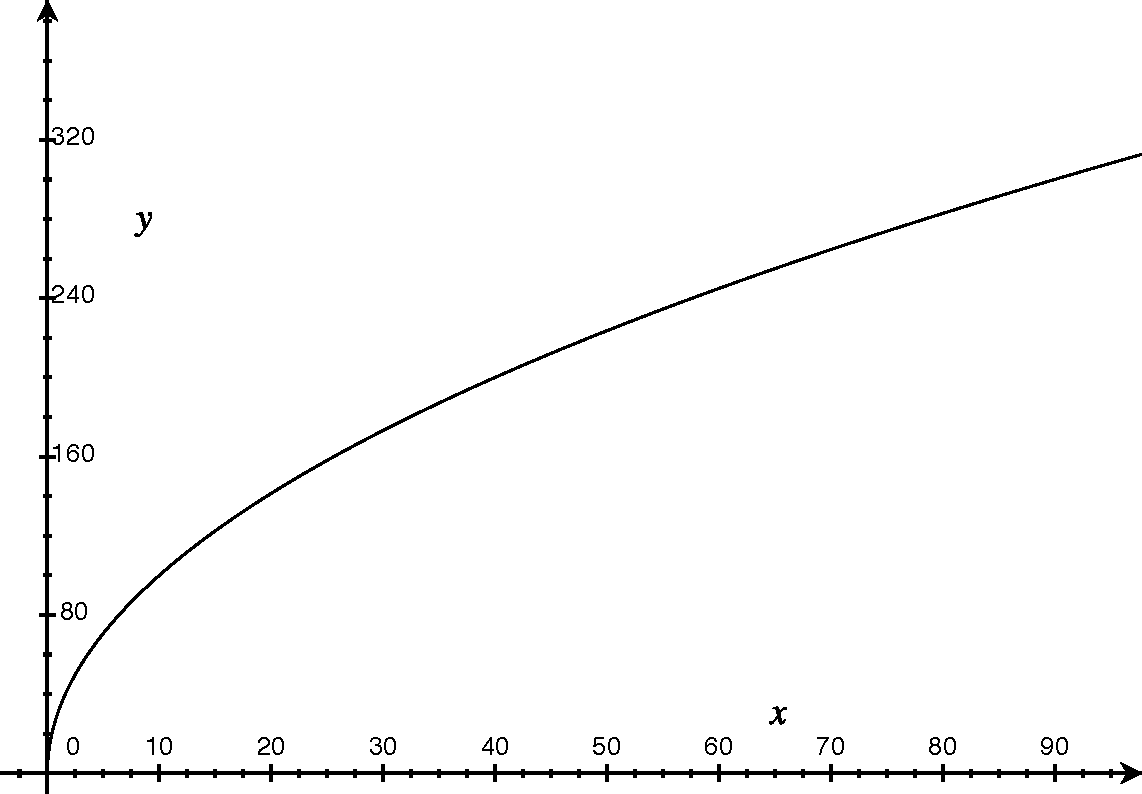
\includegraphics[width=0.6\linewidth]{./img/decutil}
\caption{Declining Marginal Utility of Money}
\label{fig:a Declining Marginal Utility of Money}
\end{figure}
\noindent You should read the $x$-axis there are measuring possible incomes in thousands of dollars per year, and the $y$-axis as measuring utility. The curve there is $y = x^{\frac{1}{2}}$. That isn't necessarily a plausible account of how much utility each income might give you, but it's close enough for our purposes. Note that although more income gives you more utility, the amount of extra utility you get from each extra bit of income goes down as you get more income. More precisely, the slope of the income-utility graph keeps getting shallower and shallower as your income/utility rises. (More precisely yet, a little calculus shows that the slope of the graph at any point is $\frac{1}{2y}$, which is obviously always positive, but gets less and less as your income/utility gets higher and higher.)

Now as you can see, that curve is rather steeping curving down. But it is common to think that in real life, the marginal utility of money diminishes even more quickly than that. Some economists think that the utility of a certain level of wealth is not best measured by the square root of that wealth level, but by the logarithm of it. On this way of thinking, multiplying your wealth by a common factor always has the same difference on your utility, whether that is taking your wealth from \$10,000 to \$100,000, or from \$1,000,000 to \$10,000,000. And some economists think that we can be satiated; that is, we can reach a point where extra material resources make no difference to utility at all. This is controversial; what is not controversial is the thesis that money has a declining marginal utility.

The fact that there is a declining marginal utility of money explains certain features of economic life. We'll look at models of two simple economic decisions, buying insurance and diversifying an investment portfolio. We'll then use what we said about diversified investments to explain some features of the actual insurance markets that we find.

\section{Insurance}
Imagine the utility an agent gets from an income of $x$ dollars is $x^{\frac{1}{2}}$. And imagine that right now their income is \$90,000. But there is a 5\% chance that something catastrophic will happen, and their income will be just \$14,400. So their expected income is $0.95 \times 90,000 + 0.05 \times 14,400 = 86220$. But their expected utility is just $0.95 \times 300 + 0.05 \times 120 = 291$, or the utility they would have with an income of \$84,861.

Now imagine this person is offered insurance against the catastrophic scenario. They can pay, say, \$4,736, and the insurance company will restore the \$75,600 that they will lose if the catastrophic event takes place. Their income is now sure to be \$85,264 (after the insurance is taken out), so they have a utility of 292. That's higher than what their utility was, so this is a good deal for them.

But note that it might also be a good deal for the insurance company. They receive in premiums \$4,736. And they have a 5\% chance of paying out \$75,600. So the expected outlay, in dollars, for them, is \$3,780. So they turn an expected profit on the deal. If they repeat this deal often enough, the probability that they will make a profit goes very close to 1.

The point of the example is that people are trying to maximise expected utility, while insurance companies are trying to maximise expected profits. Since there are cases where lowering your expected income can raise your expected utility, there is a chance for a win-win trade. And this possibility, that expected income can go down while expected utility can go up, is explained in virtue of the fact that there is a declining marginal utility of money. 

\section{Diversification}
Imagine that an agent has a starting wealth of 1, and the utility the agent gets from wealth $x$ is $x^{\frac{1}{2}}$. (We won't specify $x$ what, but take this to be some kind of substantial unit.) The agent has an opportunity to make an investment that has a 50\% chance of success and a 50\% chance of failure. If the agent invests $y$ in the scheme, the returns $r$ will be
\begin{equation*}
r = \begin{cases}4y,& \text{if success} ,\\ 0,& \text{if failure} .\end{cases}
\end{equation*}
The expected profit, in money, is $y$. That's because there is a 50\% chance of the profit being $3y$, and a 50\% chance of it being $-y$. But in utility, the expected return of investing 1 unit is 0. The agent has a 50\% chance of ending with a wealth of 4, i.e. a utility of 2, and a 50\% chance of ending with a wealth of 0, i.e. a utility of 0.

So making the investment doesn't seem like a good idea. But now imagine that the agent could, instead of putting all their money into this one venture, split the investment between two ventures that (a) have the same probability of returns as this one, and (b) their success of failure is probabilistically independent. So the agent invests $\frac{1}{2}$ in each deal. The agent's return will be
\begin{equation*}
r = \begin{cases}4,& \text{if both succeed} ,\\ 2,& \text{if one succeeds and the other fails},\\ 0,& \text{if both fail} .\end{cases}
\end{equation*}
The probability that both will succeed is $\frac{1}{4}$. The probability that one will succeed and the other fail is $\frac{1}{2}$. (Exercise: why is this number greater?) The probability that both will fail is $\frac{1}{4}$. So the agent's expected profit, in wealth, is 1. That is, it is $4 \times \frac{1}{4} + 2 \times \frac{1}{2} + 0 \times \frac{1}{4}$, i.e. 2, minus the 1 that is invested, so it is 2 minus 1, i.e. 1. So it's the same as before. Indeed, the expected profit on each investment is $\frac{1}{2}$. And the expected profits on a pair of investments is just the sum of the expected profits on each of the investments.

But the expected utility of the `portfolio' of two investments is considerably better than other portfolios with the same expected profit. One such portfolio is investing all of the starting wealth in one 50/50 scheme. The expected utility of the portfolio is $4^{\frac{1}{2}} \times \frac{1}{4} + 2^{\frac{1}{2}} \times \frac{1}{2} + 0 \times \frac{1}{4}$, which is about 1.21. So it's a much more valuable portfolio to the agent than the portfolio which had just a single investment. Indeed, the diversified investment is worth making, while the single investment was not worth making.

This is the general reason why it is good to have a diversified portfolio of investments. It isn't because the expected profits, measured in dollars, are higher this way. Indeed, diversification couldn't possibly produce a higher expected profit. That's because the expected profit of a portfolio is just the sum of the expected profits of each investment in the portfolio. What diversification can do is increase the expected utility of that return. Very roughly, the way it does this is by decreasing the probability of the worst case scenarios, and of the best case scenarios. Because the worst case scenario is more relevant to the expected utility calculation than the best case scenario, because in general it will be further from the median outcome, the effect is to increase the expected utility overall.

One way of seeing how important diversification is is to consider what happens if the agent again makes two investments like this, but the two investments are probabilistically linked. So if one investment succeeds, the other has an 80\% chance of success. Now the probability that both will succeed is 0.4, the probability that both will fail is 0.4, and the probability that one will succeed and the other fail is 0.2. The expected profit of the investments is still 1. (Each investment still has an expected profit of $\frac{1}{2}$, and expected profits are additive.) But the expected utility of the portfolio is just $4^{\frac{1}{2}} \times 0.4 + 2^{\frac{1}{2}} \times 0.2 + 0 \times 0.4$, which is about 1.08. The return on investment, in utility terms, has dropped by more than half.

The lesson is that for agents with declining marginal utilities for money, a diversified portfolio of investments can be more valuable to them than any member of the portfolio on its own could be. But this fact turns on the investments being probabilistically separated from one another.

\section{Selling Insurance}
In the toy example about insurance, we assumed that the marginal utility of money for the insurance company was flat. That isn't really true. The insurance company is owned by people, and the utility of return to those people is diminishing as the returns get higher. There is also the complication that the insurance company faces very different kinds of returns when it is above and below the solvency line.

Nevertheless, the assumption that the marginal utility of money is constant for the insurance company is constant is a useful fiction. And the reason that it is a useful fiction is that if the insurance company is well enough run, then the assumption is close to being true. By `well enough run', I simply mean that their insurance portfolio is highly diversified.

We won't even try to prove this here, but there are various results in probability theory that suggest that as long as there are a lot of different, and probabilistically independent, investments in a portfolio, then with a very high probability, the actual returns will be close to the expected returns. In particular, if the expected returns are positive, and the portfolio is large and diverse enough, then with a very high probability the actual returns will be positive. So, at least in optimal cases, it isn't a terrible simplification to treat the insurance company as if it was sure that it would actually get its expected profits. And if that's the case, the changing marginal utility of money is simply indifferent.

The mathematical results that are relevant here are what are sometimes called the ``Law of Large Numbers''. The law says that if you sample independent and identically distributed random variables repeatedly, then for any positive number $e$, the probability that the average output is within $e$ of the expected output goes to 1 as the number of samples goes to infinity. The approach can be quite quick in some cases. The following table lists the probability that the number of heads on $n$ flips of a random coin will be (strictly) between $0.4n$ and $0.6n$ for various values of $n$.

\starttab{c c}
\textbf{Number of flips} & \textbf{Probabiilty of between} $\mathbf{0.4n}$ \textbf{and} $\mathbf{0.6n}$ \textbf{heads} \\ 
1 & 0 \\
10 & 0.246 \\
20 & 0.497 \\
50 & 0.797 \\
100 & 0.943 \\
200 & 0.994 \\
500 & $>$ 0.99
\stoptab This depends crucially on independence. If the coin flips were all perfectly dependent, then the probabilities would not converge at all.

Note we've made two large assumptions about insurance companies. One is that the insurance company is large, the other is that it is diversified. Arguably both of these assumptions are true of most real-world insurance companies. There tend to be very few insurance companies in most economies. More importantly, those companies tend to be fairly diversified. You can see this in a couple of different features of modern insurance companies. 

One is that they work across multiple sectors. Most car insurance companies will also offer home insurance. Compare this to other industries. It isn't common for car sales agents to also be house sales agents. And it isn't common for car builders to also be house builders. The insurance industry tends to be special here. And that's because it's very attractive for the insurance companies to have somewhat independent business wings, such as car insurance and house insurance.

Another is that the products that are offered tend to be insurance on events that are somewhat probabilistically independent. If I get in a car accident, this barely makes a difference to the probability that you'll be in a car accident. So offering car insurance is an attractive line of business. Other areas of life are a little trickier to insure. If I lose my home to a hurricane, that does increase, perhaps substantially, the probability of you losing your house to a hurricane. That's because the probability of their being a hurricane, conditional on my losing my house to a hurricane, is 1. And conditional on their being a hurricane, the probability of you losing your house to a hurricane rises substantially. So offering hurricane insurance isn't as attractive a line of business as car insurance. Finally, if I lose my home to an invading army, the probability that the same will happen to you is very high indeed. In part for that reason, very few companies ever offer `invasion insurance'.

A lot of the financial crisis in the late 2000s was related to a similar problem. A lot of the financial institutions that failed were selling, either explicitly or effectively, mortgage insurance. That is, they were insuring various banks against the possibility of default. One problem with this is that mortgage defaults are not probabilistically independent. If I default on my mortgage, that could be because I lost my job, or it could be because my house price collapsed and I have no interest in sustaining my mortgage. Either way, the probability that you will also default goes up. (It goes up dramatically if I defaulted for the second reason.) What may have been sensible insurance policies to write on their own turned into massive losses because the insurers underestimated the probability of having to pay out on many policies all at once.